\clearpage
\chapter{Introduction}
\label{sec:intro}

Performing experiments is a key component of human development and has been the foundation of knowledge gain during the evolution of mankind. However, the exchange of such experimental results requires the long term documentation of the  experimental procedure. This is only possible with the means of writing down the experimental purpose, execution and result since the invention of scripture. Nowadays, tideous manual scripture has largely been replaced by digital information, making information easier transportable, searchable and duplicatable. Therefore all scientific research nowadays relies mainly on digital information acquisition and storage. Although data can be easily stored and transferred with modern technologies, interpretation of research data is not straight forward as datasets are highly diverse between scientific areas. Depending on the area of research, the diversity within a field highly depends on the field, e.g. in fields which require large experimental setups (particle physics / high field FMRI) data formats and structures  there are only a few data formats defined by the community / company producing the corresponding setup. In other fields the diversity of data is bigger since the scientific methods and aims require a diversity of approaches. Unification would require organizational large-scale efforts arcoss the community and implies additional overhead on the level of each experiment. In this thesis I discuss approaches for data and metadata management for efficient and robust handling of research data from data aquisition to analyis.

The diversity in data modalities and file formats promotes also a heterogeneity in data analysis steps and tools used for extraction of scientific findings.

\todo{TODO: go on here with describing need to standardize analyses and the requirement of complete / consistent metadata}
\todo{Introduce: Reproducible vs replicable vs ...}

\todo{Introduce odML, nix, ...}


\section{Data and metadata models}
Standardization of data and metadata is a fundamental requirement for the usability of data and metadata. This work is based on two common, generic models for capturing metadata and data. Both software projects are developed and maintained by the German Neuroinformatics Node (G-Node) an organization aiming to improve the infrastructure for data access, data storage and data analysis. 

\subsection{Hierarchical metadata in the \software{odML} model}
\label{sec:subodML}

odML\footnote{\url{https://github.com/G-Node/python-odml}, RRID:SCR\_001376} is a versatile hierarchical format for metadata \citep{Grewe_2011} developed by the German Neuroinformatics Node (G-Node). While it was originally designed for electrophysiological metadata, its generic structure makes it also applicable to other scientific contexts.

The basic concept is to use a tree-like structure of \textbf{Sections} to store metadata as \textbf{Properties} (extended key-value pairs) in a common \textbf{Document} (\cref{fig:odml_versions}B). For example, using this paradigm,  parameter settings of a specific device used in the experiment would be represented as Properties collected in a specific Section for that device. For a detailed tutorial\footnote{\url{https://github.com/G-Node/python-odml/blob/master/doc/tutorial.rst}} on \software{odML} please refer to the online reference documentation\footnote{\url{http://g-node.github.io/python-odml}}. The usage of \software{odML} in different environments with varying requirements has led to diversification, the identification of unused features, and the need for improvement of the original data model. In case of the \software{odMLtables} project, for example, the original internal data representation required only a subset of the complete \software{odML} data model. These and other re-implementations (NIX and RELACS projects) did not fully comply with the original specifications and led to a diversification of the de-facto implemented data models. In order to resolve this situation, with the latest release of \software{odML} version 1.4\footnote{\url{https://github.com/G-Node/python-odml/releases/tag/v1.4.0}} (i) data model and implemented features were streamlined and adapted to ensure compatibility between the various project implementations and (ii) additional features were introduced. The following paragraph briefly reviews the changes of the data model since its publication in \cite{Grewe_2011}.


\begin{figure}
    \centering
    \includestandalone[mode=image|tex, width=\textwidth, obeyclassoptions=true]{./figures/introduction/odML_structure}
%     \include[width=\textwidth,pretex=\relscale{0.8}]{./figures/neo07_schema.svg}
    \caption[Neo embedding]{\software{Neo} embedding. \software{Neo} 0.7. supports a number of file formats for reading (light blue) and writing (dark blue). Many of the supported formats can be read in a improved fashion, permitting for more efficient memory usage (black frames).  Neo provides an interface for many advanced tools for visualization, simulation, analysis and data storage.}
    \label{fig:neo_ios}
\end{figure}

\paragraph{\software{odML} model revision and streamlining}
\label{sec:odml_model_revision}
A number of features were merged or moved by the change from \software{odML} version 1.3 to version 1.4 in order to simplify usage of the \software{odML} framework as originally described in \citet{Grewe_2011}, and to mitigate potential ambiguities in the data structure. In the following, we briefly explain two major changes that affected the design and use of odMLtables. The first change was the merging of Value and Property entities (compare \cref{fig:odml_versions} A and B). This prevents value ambiguities within a Property and reduces the effective file size since the value dependent attributes ("unit", "uncertainty", "data type" and "reference") are defined only once for a set of values. This change simplified also the tabular representations of lists of values created by odMLtables. Second, for compatibility with the NIX projects' \software{odML} implementation, entities now contain a universally unique identifier (UUID, auto-generated identifier with extremely low collision probability) for unique identification of \software{odML} entities even across unrelated files to ensure comprehensive provenance tracking, including the ability to create tabular metadata representations across projects using future \software{odMLtables} versions. Compatibility for \software{odML} files using the old format version is ensured via automatized conversion functionality.
\todo{Add paragraph about empty list of values now being possible, for reference in scidata\_odmlgeneration workflow}

\begin{figure}
    \centering
    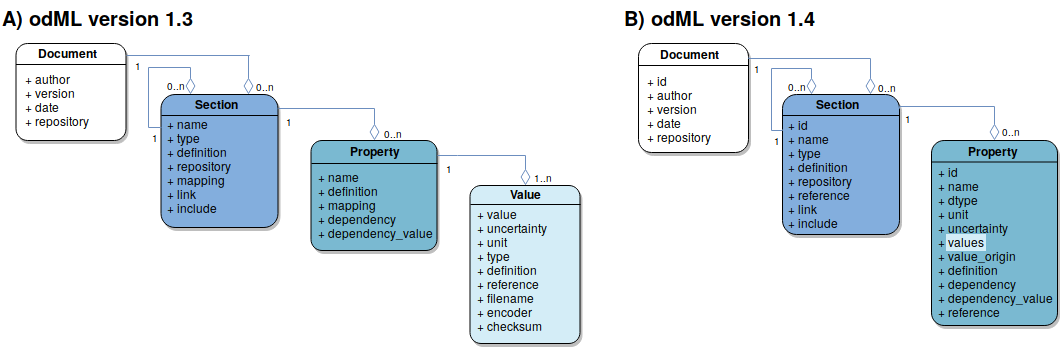
\includegraphics[width=1.0\columnwidth]{figures/odmltables_figures/fig3_odml_data_model/odML_DataModel_version.png}
    \caption[Evolution of the \software{odML} data-model]{\textbf{Evolution of the \software{odML} data-model.} Each box represents an entity defined by the data model and is color coded. Connections between entities are illustrated using the UML aggregation relation where a diamond denotes the target of a connection; the numbers at source and target denote the cardinality of each entity in the connection. (A) Version 1.3 data model. Four entities are defined: The \textit{Document} (marked in white) as the root element of a metadata file contains information about the author, document date, the document version and a default repository containing definitions used within the Document. It further contains grouping elements, \textit{Section}s (marked in dark blue). These are defined via their name and type attributes and can hold Subsections and provide semantic structure to an \software{odML} Document. The "definition" attribute provides information about the nature of a Section, while "link" and "include" refer to further Sections within the same or a different Document, respectively. Sections may contain named \textit{Property} entities (marked in cyan) which hold at least one \textit{Value} (marked in light blue) thus creating an extended key-value pair. (B) Version 1.4 data model: To simplify the use of the \software{odML} data model the Value entity was integrated into the Property taking over the attributes "dtype" (data type), "unit", "uncertainty", "value origin", and "reference". In this version a Property may contain a list of values, which must be identical in terms of the relocated attributes thus reducing the risk of ambiguities in the value list. For more information on attributes that have not been modified please refer to the original publication \citep{Grewe_2011}. Figure with permission adapted from \cite{Grewe_2011}.}
    \label{fig:odml_versions}
\end{figure}

\paragraph{Additional features}
The \software{odML} core library already provides an in-built mechanism to search and retrieve Sections, Properties or values within a Document. The need to consistently search for metadata entities across Documents from different sources led to the development of an export feature of \software{odML} metadata to the Resource Description Framework (RDF) format\footnote{\url{http://www.w3.org/TR/rdf-primer}}, a general and widely used storage format of graph databases. Multiple \software{odML} files exported to RDF can be loaded into any graph database supporting RDF and will be combined into a single graph. Moreover, while XML is still the default storage format, \software{odML} now additionally supports storing the metadata in the text based file formats JSON\footnote{\url{https://json.org}} and YAML\footnote{\url{https://yaml.org}}. JSON has become a de-facto data exchange standard between web based and standalone computer applications. The support of JSON makes \software{odML} metadata more easily consumable in machine-only workflows through modern applications. Since both XML and JSON primarily aim at machine-readability, their structure is not easily readable by humans. To ease reading of raw \software{odML} files by actual persons the YAML file format support was added.

For easy visualization and manipulation of specific \software{odML} files, the graphical user interface of \software{odMLtables} was integrated into the native \software{odML} GUI (odml-ui\footnote{\url{https://github.com/G-Node/odml-ui}}). Thus, the \software{odML} GUI now grants direct access to the main \software{odMLtables} features, making both software tools even easier to use back to back for both browsing and editing of metadata.


\subsection{Generic data organization via the \software{Nix} model}
The \software{Nix} model combines data and metadata in a common framework. For this six generic data objects are defined and combined with an \software{odML} based metadata structure. The \software{Nix} model is provided with a \software{C++} reference implementation\footnote{nixio \software{C++}, \url{https://nixio.readthedocs.io},  RRID:SCR\_016196} and bindings for \software{Java}, \software{Matlab}. An independent implementation in \software{Python} is provided\footnote{nixio / nixpy, Python, \url{https://pypi.org/project/nixio/}} with version $1.5.0b3$ being considered here.

The \software{Nix} model consists of two different types of object for the description of data and metadata. In total, there are six data and two metadata objects  described in the following (\ref{fig:intro_nix_model}).
Data values are caputured using \code{DataArray}s capable of holding any type of data that can be described using a single or multidimensional array. In addition to the values the \code{DataArray} also describes the physical properties of the stored values, e.g. the type of data, the physical unit of the values and a human readable label. Additionally the data array is connected to \code{Dimension} objects, providing details about each of the additional dimensions of the \code{DataArray} including also a label, the physical unit, a sampling interval and offset. With these two objects \software{Nix} captures all required data for a meaningful visualization of the stored data values (e.g. see \cref{fig:intro_nix_examples}). In addition, it offers objects for tagging subsets of the values stored in a \code{DataArray} and for describing the origin of the recording data. The first one is implemented as a \code{Tag} object, referencing a subset of the values in a \code{DataArray} and can be used to provide more information for a subset of values, e.g. the presentation of a stimulus or the labelling of a cell part. The second object is a \code{Source} object, which is used to track the origin of data. The remaining data object \code{Group} is used for logical grouping of other \software{Nix} data objects. All data objects are coordinated via \code{Block}, which again is together with the metadata objects grouped in a \software{Nix} \code{File} object, representing a complete dataset.
The metadata objects used in the \software{Nix} framework are taken from the \software{odML} framework. All data objects within \software{Nix}, except for the \code{Dimension} object, can link to a single \code{Section} in the metadata collection of the \software{Nix} \code{File}, which contains additional information about the data object. Depending on the declared types of the linked data and metadata object, this relation is interpreted mono- or bidirectional, i.e. the metadata \code{Section} enriches the data object or the metadata object is additionally also defined via the data object.

The \software{Nix} repository is accompanied with an extensive wiki\footnote{\software{Nix} wiki, \url{https://github.com/G-Node/nix/wiki}} and documentation\footnote{\software{Nix} documentation, \url{https://nixio.readthedocs.io}} including tutorials and demos, providing a simple start for new users.

The \software{Nix} model is natively integrated in the the electrophysiology recording system \software{RELACS}, the \software{EEGbase}\footnote{EEGbase, \url{http://eegdatabase.kiv.zcu.cz}, RRID:nif-0000-08190} a system for storage, management, sharing and retrieval of EEG data as well as \software{Neo}, a Python tool for standardized representation of electrophysiology data (\ref{sec:neo}).


\begin{figure}
 \centering
 \begin{minipage}[t]{0.8\textwidth}
 \textbf{A}\newline\\
 \hfill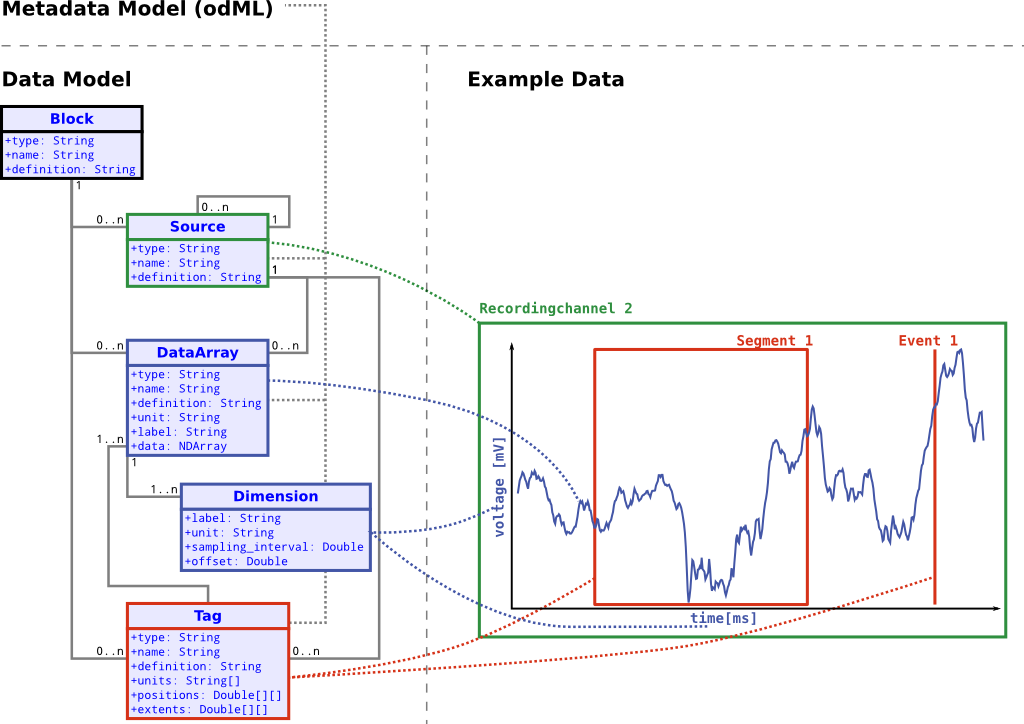
\includegraphics[width=0.9\textwidth]{./figures/introduction/pandora_example_signal}
 \end{minipage}\\
 \vspace{1cm}
 \begin{minipage}[t]{0.8\textwidth}
 \textbf{B}\newline\\
 \hfill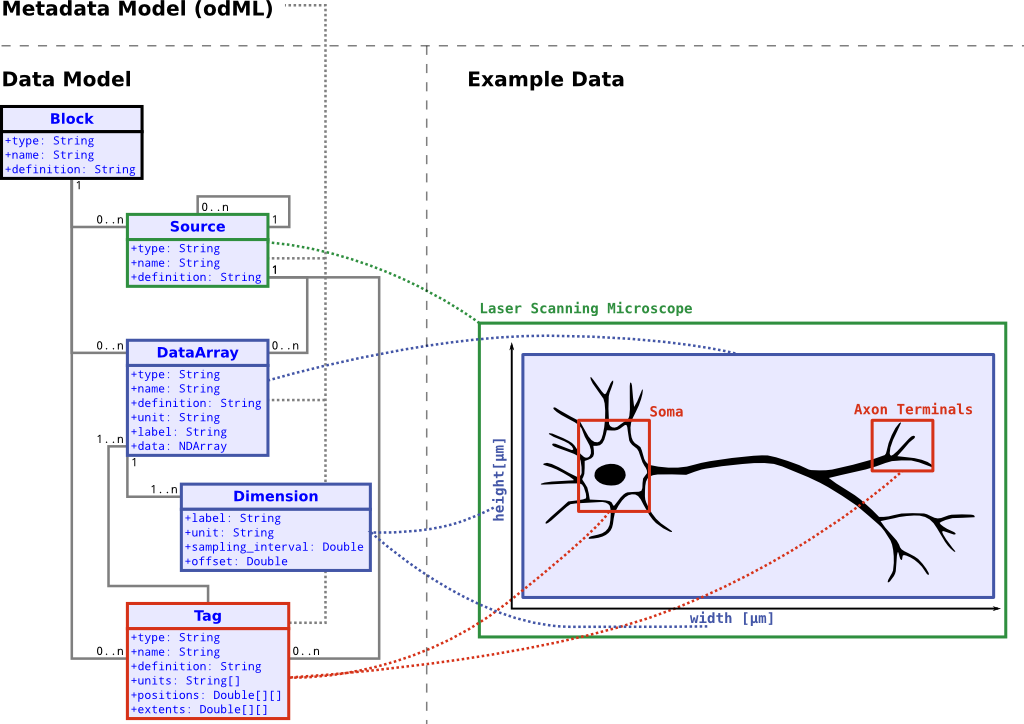
\includegraphics[width=0.9\textwidth]{./figures/introduction/pandora_example_image}
 \end{minipage}
 \caption[Nix model application examples]{Nix model application examples. The model can capture different varieties of data, e.g. electrophysiological recording traces (A) and imaging data (B). Both signals types can be mapped to the same types of objects of the \software{Nix} model. Figure from \software{Nix} documentation\footnote{\url{https://github.com/G-Node/nix/wiki/The-Model}}}
 \label{fig:intro_nix_examples}
\end{figure}

\begin{figure}
 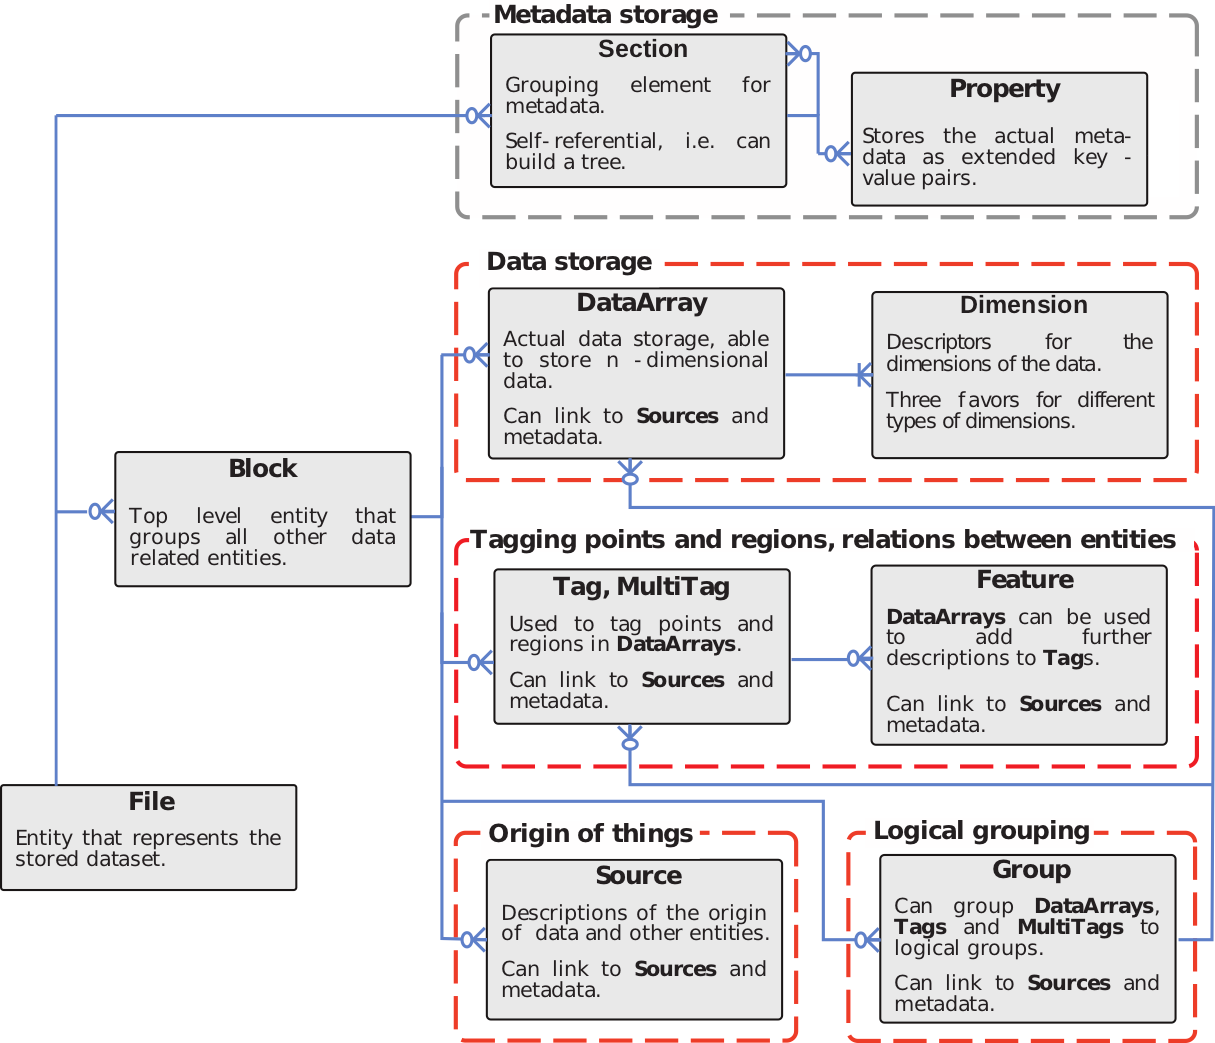
\includegraphics[width=0.9\textwidth]{./figures/introduction/data_model_brief_adapted}
 \caption[Nix model objects]{Nix model objects. The model consist of objects for storing data and metadata and relations between these. Metadata is captured in a \software{odML} based structure. Figure adapted from \software{Nix} documentation\footnote{\url{https://nixio.readthedocs.io/en/latest/data_model.html}}}
 \label{fig:intro_nix_model}
\end{figure}

\section{Thesis overview}
In \cref{sec:data} we describe two published datasets of a complex, collaborative electrophysiological experiment including an extensive metadata collection. We describe the process of data and metadata preparation required for the data publication and discuss the workflow used in this publication to identify strengths and shortcomings of the presented approach. In \cref{sec:metadata} we present odMLtables, a tool for facilitation of metadata collection compatible with the previously presented workflow. We demonstrate the embedding of odMLtables in a real-world metadata workflow and highlight the latest features and developments of the tool. \cref{sec:neo} complements the the previous section by introducing tools for standardized data representation and presents three example applications. \cref{sec:workflows} introduces modern workflow management software for efficient organization and structuring of scientific projects. We demonstrate the integration of the previously presented tools in a systematic fashion using modern workflow management software to coordinate the application of data and metadata software in a neuroscientific project. Finally, in \cref{sec:discussion} we discuss the presented approaches and provide an outlook on future development of the tools and concepts.




